%%%%%%%%%%%%%%%%%%%%%%%%%%%%%%%%%%%%% BEGIN HEADERS %%%%%%%%%%%%%%%%%%%%%%%%%%%%%%%%%%%%%%%%%%%%%%%%%%%%%
\documentclass[11pt,conference]{IEEEtran}

\usepackage{longtable}
\usepackage{graphicx}
\usepackage[utf8]{inputenc}
\usepackage{fancyhdr}
\usepackage{float}
\usepackage[hidelinks]{hyperref}
\usepackage{listings}
\usepackage{color}
\usepackage{natbib}

% Your names in the header
\pagestyle{fancy}
\rhead{Enrico Tedeschi}
\lhead{INF-3201 Parallel Programming - Assignment 2}
\cfoot{\thepage}

% Used for including code in a stylized manner
\definecolor{codegreen}{rgb}{0,0.6,0}
\definecolor{codegray}{rgb}{0.5,0.5,0.5}
\definecolor{codepurple}{rgb}{0.58,0,0.82}
\definecolor{backcolour}{rgb}{0.95,0.95,0.92}
 

\lstdefinestyle{mystyle}{
    backgroundcolor=\color{backcolour},   
    commentstyle=\color{codegreen},
    keywordstyle=\color{magenta},
    numberstyle=\tiny\color{codegray},
    stringstyle=\color{codepurple},
    basicstyle=\footnotesize,
    breakatwhitespace=false,         
    breaklines=true,                 
    captionpos=b,                    
    keepspaces=true,                 
    numbers=left,                    
    numbersep=5pt,                  
    showspaces=false,                
    showstringspaces=false,
    showtabs=false,                  
    tabsize=2
}

\lstset{style=mystyle}

% The Title
\title{INF-3201 Parallel Programming
\newline
Shared Memory}

% Your name and email
\author{\textbf{Enrico Tedeschi}\\ ete011@post.uit.no }


%%%%%%%%%%%%%%%%%%%%%%%%%%%%%%%%%%%%% END HEADERS %%%%%%%%%%%%%%%%%%%%%%%%%%%%%%%%%%%%%%%%%%%%%%%%%%%%%

\begin{document}

% Create the title and everything
\maketitle

\section{Introduction}
The goal of this assignment is to parallelize a piece of code using shared memory techniques preferably using \textbf{OpenMP}.
\newline
The piece of code to parallelize could be the given one, that is a Markovian chess engine, or a chosen piece of code which has to be approved by the professor.
\subsection{Requirements}
\begin{itemize} 
\item Choose a piece of software to parallelize
\item Parallelize it with shared-memory techniques
\item Evaluate speed up
\end{itemize}

\section{Technical Background}

\begin{itemize} 
\item[--] Concurrency and parallelism concepts
\item[--] Parallel programming concepts
\item[--] Basic programming approach
\item[--] Knowledge of C language
\item[--] Notion of design pattern principles
\item[--] Theory about software engineering
\item[--] Knowledge of git to manage the software versions
\end{itemize}


\section{Analysis}
The given \textbf{Markovian} code was found to be too long and quite hard to understand, in addition, it has no deterministic solution so it would have been really difficult to test.
\newline
The code chosen to be parallelized is a sequential version of the \textbf{TSP} (Traveller Salesman Problem). It asks the following question: \textit{Given a list of cities and the distances between each pair of cities, what is the shortest possible route that visits each city exactly once and returns to the origin city?} \cite{citation1}
\newline
The sequential code was refined by adding a random function which generate distances between cities and also the possibility of run the programme with a size passed as a parameter was implemented.
\newline
To parallelize a sequential code is necessary to analyse which function involves the biggest amount of time. The c given program \textit{tsp-seq.c} has been tested with \textit{profile} and the following table is the result of this test:
\begin{lstlisting}
  %   cumulative   self               
 time   seconds    calls   name    
100.32   2.90        1     zRoute
  0.00   0.00      196     zEuclidDist
  0.00   0.00       28     random_at_most
  0.00   0.00        2     second
  0.00   0.00        1     zReadRoute
\end{lstlisting}

the function to parallelize is obviously \textit{zRoute}.
\newline
The function has a recursive structure for each possible successor of the city chosen as initial. For instance, if the function would have a $iSize = 5$ (number of cities) then the execution tree would look like the one in Fig \ref{fig:tree}. 
In the first 'level' of the tree the first city executes recursively the $zRoute$ function for the number of the cities left to visit, and so for the other levels.
Having an image of the execution tree helps to get the parallelization easier.
\begin{figure}[h!]
  \centering
    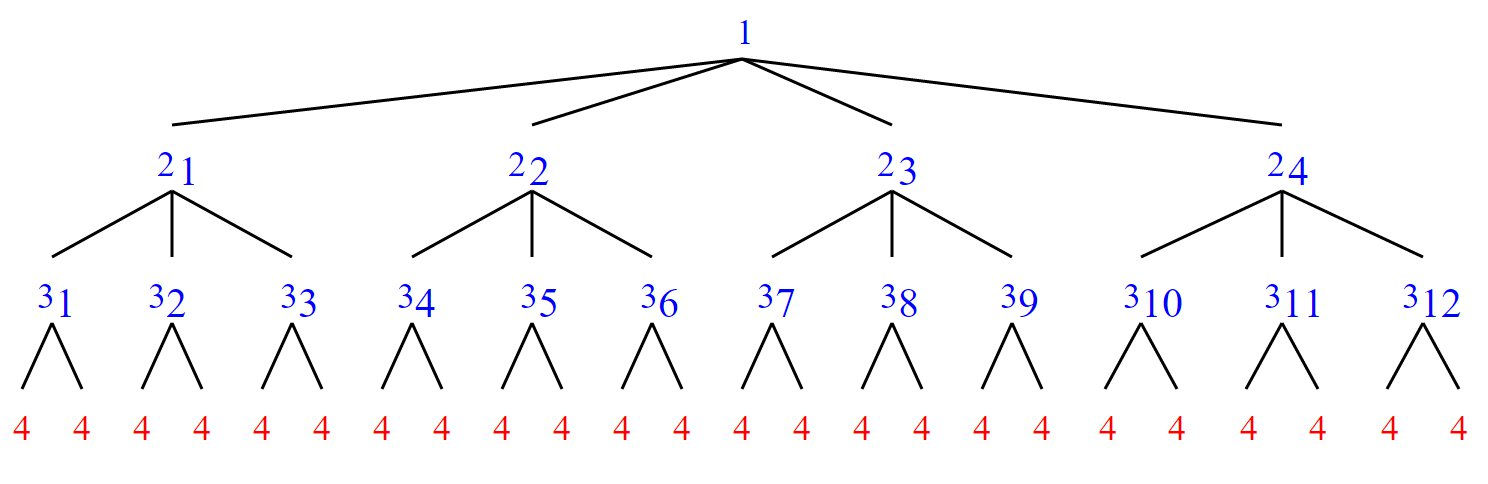
\includegraphics[width=0.5\textwidth]{tree}
    \caption{Execution of the zRoute function}
    \label{fig:tree}
\end{figure}

\section{Implementation}
\subsection{Environment}
The code has been developed using JetBrains CLion 1.1 on Windows 10 and due to a more easy way to compile and test the MPI programs with a Linux based console, the compilation and the execution of the code has been made on an Ubuntu Virtual Machine with 4 core assigned, using VirtualBox 4.2 and Ubuntu version 14.04.3
\newline
To synchronize the cluster and the local machine and to keep trace of all the changes in the code, a git repository was created and the git command on linux were used to commit and to push/pull data from repositories.
\newline
The benchmarking and the test with more than 4 cores has been done in the UiT uvrocks cluster. The connection with the cluster was established by using ssh on a linux machine:
\begin{lstlisting}
ssh -X -A ete011@uvrocks.cs.uit.no
\end{lstlisting}
To simplify the execution of the code, a proper Makefile was implemented.

\subsection{Fixing the Sequential Version}
Before starting the parallelization some changes to the sequential version were implemented. The way to verify if the solution found is reliable is to check the $length$ of the path to visit all the cities. The length of the path changes if either the number of cities or the size of the map is changed, but it's not dependent from where the cities are located. Considering that, a function which generates random numbers from \textit{0 to max\_size} is created, so every time, given a number of cities and a max\_size defined, is possible to generate random coordinates for the cities which won't influence the correct $crc$ anyway.
The sequential version, \textit{tsp-seq.c}, takes as input the number of cities and it has a fixed map size.

\subsection{Approaching the Problem}
Due to the tricky recursive function the first goal of the implemented parallelization was: "get the speed up keeping the code simple". 
The Fig \ref{fig:tree-par} shows the logic used for the parallelization. The parts of the tree enhanced in red are the component which will run in parallel; in that way the speed up is strongly dependent from the relation between the $number\_of\_cores$ and the $number\_of\_cities$. Using this kind of approach the parallelization is made in the first $for$ cycle, and each core will execute the recursive function, solving all the sub-branches problems related to it.

\begin{figure}[h!]
  \centering
    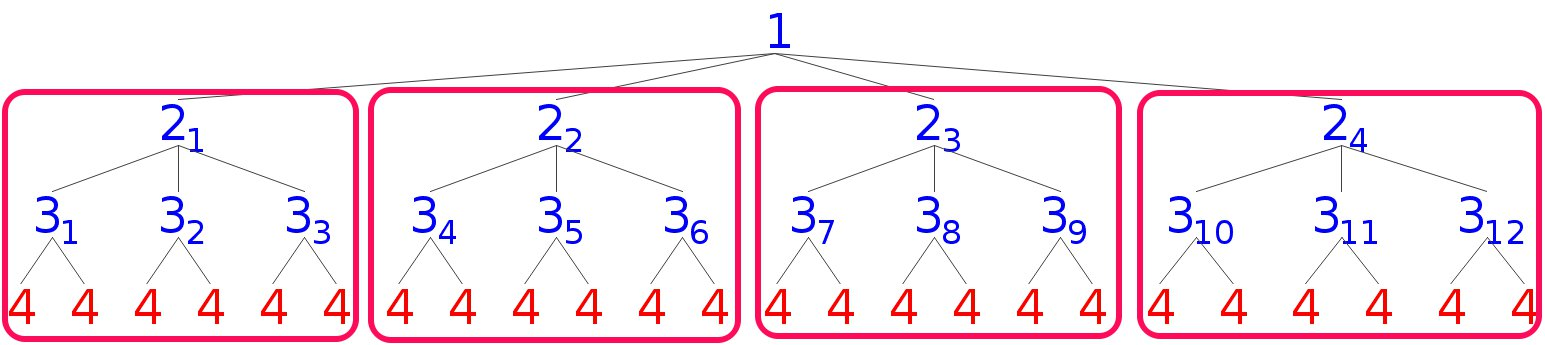
\includegraphics[width=0.5\textwidth]{tree-par}
    \caption{Execution of the parallel version of the zRoute function, with 5 cities using 4 parallel cores}
    \label{fig:tree-par}
\end{figure}

\subsection{Parallelization}
For the parallelization \textbf{OpenMP} API were used. They provide to standardize directive-based multi-language high-level parallelism that is performant, productive and portable\cite{citation4}. Since the $zRoute$ function is recursive is necessary to define two types of $zRoute$ functions, a \textbf{sequential} one and a \textbf{parallel} one. If the code is in the first level of the tree, then it will call for each sub-branches the recursive parallel function, otherwise it will call the sequential one.
\newline
The biggest problem to solve was related to shared memory and how the variables were used while parallelizing the code. OpenMp indeed takes care about the balancing of the work but is necessary to have well defined which variable needs to be global and which ones local.
\newline
To parallelize the function the following logic was used:
\begin{lstlisting}
count = 0;
void zRoute(...){
    if (count == 0) {
    	count++;
    	#pragma omp parallel num_threads(#)
    	{
    	#pragma omp for
    	--core of zRoute function--
    	}
    }
    else{
    	--core of zRoute function--
    }
    return;
}
\end{lstlisting}

To keep the variables local, a strong analysis on them has been done. All the variables which change their value during the execution (called $var\_c$ in the listing below) of zRoute must have been declared locally. To achieve that, a function called \textit{for\_cycle\_zRoute} has been created and it is called only when $count = 0$, that is  when the code needs to be parallelized. Therefore the function it receives as input all these variables which need to be locally declared and it executes the core of the zRute function.

\begin{lstlisting}
void zRoute(...){
    if (count == 0) {
    	#pragma omp parallel num_threads(#)
    	{
    		for_cycle_zRoute(var_c);
    	}
    }
    else{
    	--core of zRoute function--
    }
    return;
}
\end{lstlisting}

The logic for the \textit{for\_cycle\_zRoute} function is:

\begin{lstlisting}
void for_cycle_zRoute(var_c){
    --definition of local variables--
    #pragma omp for
    --core of zRoute function--
    return;
}
\end{lstlisting}
\section{Result and Benchmarking}
For the benchmarking the parallel
%TODO: benchmarking with speed up and with efficency
%TODO: scale with number of cities: compare sequential one with fixed parallel threads one.
%TODO: scale with number of threads: compare sequential (eg 16 cities) with parallel using 1--16, 20,30,40 threads
%TODO: compare with the sequential one
%TODO: talk about of not having used the omp profiling

\section{Discussion}

%TODO: Talk about that is possible to parallelize more when n_cores >> n_cities
%TODO: A possible optimization is to check if the n_cores >> n_cities if yes then divide the work one level down or create a pull of works for each recursive call and the threads are going to take the work from there.
%TODO: With an high number of cities the speedup is not gonna be so much better than the sequential one, because executing the zRoute function is a exponential problem

\section{Conclusion}

%TODO: which speedup achieved
%TODO: Considering the few days of work I can consider satisfied for the work done

\bibliographystyle{plain}
\bibliography{report}


\end{document}

